La fase di prototipazione a bassa fedeltà ha avuto lo scopo di esplorare rapidamente l'architettura dell'applicazione prima di vincolarla a una forma definita.
Tutte le schermate sono state disegnate a mano libera con Excalidraw su un unico foglio, così da mantenere simultaneamente visibili le interfacce, le frecce che ne descrivono le transizioni e le annotazioni a margine in cui sono state fissate le motivazioni delle singole scelte.
Il livello di dettaglio, deliberatamente approssimativo nelle proporzioni e privo di qualsiasi indicazione cromatica, ha permesso di concentrare il ragionamento sulla presenza e sulla gerarchia degli elementi anziché sul loro aspetto, riducendo al minimo il costo di scartare un'idea rivelatasi inadeguata.

L'esplorazione non si è limitata a variare posizione e dimensione dei componenti all'interno di una stessa schermata, ma ha messo a confronto due modi opposti di intendere l'applicazione.
Il primo la riduce al solo gesto di emergenza, con una schermata principale occupata dal pulsante di aiuto e da nulla che possa distrarne la lettura.
Il secondo la concepisce come uno strumento di accompagnamento quotidiano, in cui il gesto di emergenza convive con il tracciamento dell'umore, con le attività avviabili in autonomia e con la sintesi dei progressi.
La tensione fra i due approcci discende direttamente dai requisiti: l'esigenza di un'interfaccia minimale e a basso carico cognitivo (\textbf{REQ-01}) spinge verso lo svuotamento della schermata, mentre il tracciamento emotivo (\textbf{REQ-06}), l'accesso autonomo agli esercizi (\textbf{REQ-08}) e la restituzione dell'andamento settimanale (\textbf{REQ-09}) richiedono che l'applicazione abbia qualcosa da offrire anche quando l'utente sta bene.

Nei paragrafi seguenti le schermate vengono presentate una per una, esplicitando per ciascuna la funzione assolta e le alternative valutate.
Dove il confronto ha individuato una soluzione nettamente più coerente con i requisiti, la proposta meno efficace è stata scartata e la decisione motivata.
Dove invece nessuna delle due si è imposta sull'altra, entrambe sono state conservate e tradotte in wireframe digitali, per essere sottoposte alla valutazione empirica con gli utenti.
Alcune schermate di servizio, infine, non presentano alternative concorrenti, poiché l'aderenza alle convenzioni consolidate costituisce in quei casi il risultato desiderato.

\section{Schermata di accesso: login e creazione account}
\label{sec:sketch-accesso}

L'area di accesso è stata la prima porzione di interfaccia affrontata in fase esplorativa, poiché costituisce il punto in cui l'utente incontra l'applicazione e, allo stesso tempo, quello in cui il progetto rischia maggiormente di contraddire il requisito di accesso immediato senza barriere all'ingresso (\textbf{REQ-04}).
Lo sketch adotta deliberatamente un'impostazione convenzionale, con il modulo delle credenziali, il recupero della password e il rimando alla registrazione collocato in fondo alla schermata.
La scelta non deriva dall'assenza di alternative, ma dalla convinzione che il modulo di autenticazione non sia il luogo in cui sperimentare soluzioni originali: un layout riconoscibile a colpo d'occhio viene attraversato senza doverci ragionare sopra, condizione tanto più necessaria quanto minore è la lucidità della persona che lo sta usando (\textbf{REQ-01}).

La decisione di progetto vera e propria riguarda il comando per continuare come ospite, collocato immediatamente sotto il pulsante di accesso e introdotto dalla congiunzione \enquote{oppure}.
La formulazione presenta le due strade come equivalenti anziché suggerire un ripiego, mentre la posizione nella metà inferiore della schermata la rende raggiungibile senza modificare la presa sul dispositivo.
L'obiettivo è rimuovere il registration wall individuato come ostacolo principale nell'analisi dei competitor, evitando che una persona in difficoltà sia costretta a compilare un modulo prima di poter raggiungere gli strumenti di soccorso (\textbf{REQ-04}).

\begin{figure}[htbp]
    \centering
    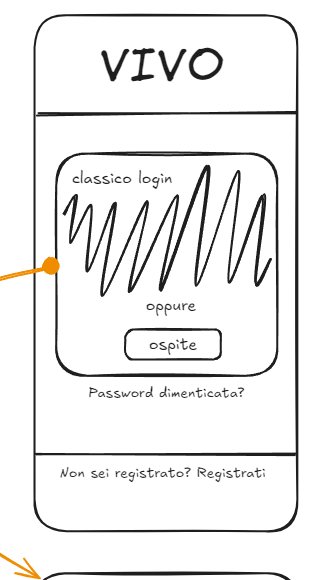
\includegraphics[height=8cm]{imgs/sketches/login-s.png}\hspace{1cm}
    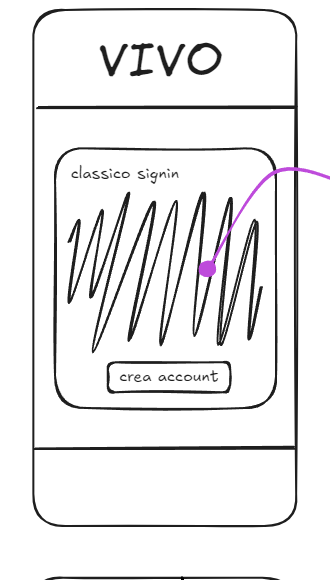
\includegraphics[height=8cm]{imgs/sketches/registrazione-s.png}
    \caption{Sketch dell'accesso e della creazione dell'account}
    \label{fig:sketch-accesso}
\end{figure}

La creazione dell'account è stata invece isolata in una schermata dedicata, raggiungibile dal rimando in fondo alla pagina di accesso e mai presentata all'avvio.
Questa gerarchia mantiene la registrazione a disposizione di chi desidera conservare il proprio storico nel tempo (\textbf{REQ-07}), senza però anteporla all'uso dell'applicazione: i dati anagrafici vengono richiesti soltanto nel momento in cui l'utente ha già scelto di volere un profilo, secondo il principio per cui un'informazione va chiesta quando diventa pertinente e non prima.
L'annotazione a margine dello sketch si limita del resto a registrare la necessità di raccogliere le informazioni personali per la creazione dell'account, senza prevedere alcuna procedura di configurazione da attraversare prima di poter usare l'applicazione.

Nessuna delle due impostazioni presenta alternative concorrenti da mettere a confronto, trattandosi di schermate di servizio in cui l'aderenza alle convenzioni è essa stessa il risultato desiderato.
Entrambe sono state pertanto trasferite direttamente alla fase di wireframing, dove sono state arricchite con i riscontri visivi sui campi e con il messaggio esplicito sul trattamento locale dei contenuti (\textbf{REQ-05}).

\section{Schermata principale: dashboard di supporto emotivo}
\label{sec:sketch-principale}

La schermata principale è il punto in cui l'identità dell'applicazione si dichiara per intero, e le due alternative disegnate in fase esplorativa incarnano con particolare nettezza i due approcci contrapposti descritti in apertura di capitolo.
La questione da risolvere non riguardava la disposizione dei componenti, ma la natura stessa dello strumento: un dispositivo di emergenza da aprire soltanto durante una crisi, oppure un compagno quotidiano che accompagna l'utente anche nei periodi di calma.

\begin{figure}[htbp]
    \centering
    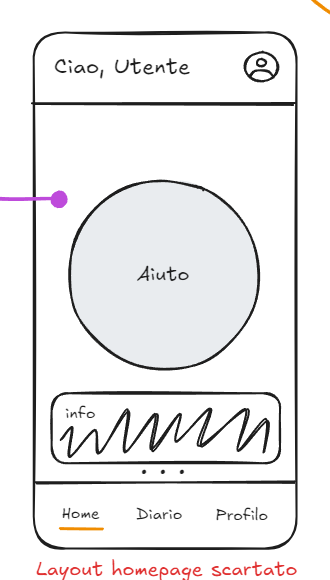
\includegraphics[height=8cm]{imgs/sketches/homepage-alt-s.png}\hspace{1cm}
    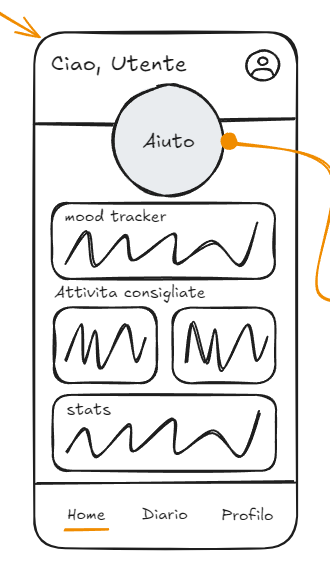
\includegraphics[height=8cm]{imgs/sketches/homepage-s.png}
    \caption{Le due idee di schermata principale messe a confronto: il solo gesto di emergenza e la dashboard quotidiana}
    \label{fig:sketch-homepage}
\end{figure}

La prima variante riduce la schermata al solo gesto di soccorso.
Un unico pulsante circolare di grandi dimensioni occupa il centro dell'interfaccia, accompagnato in basso da una fascia informativa scorrevole segnalata da indicatori di pagina.
Il vantaggio è evidente e riguarda direttamente il requisito di un'interfaccia minimale e a basso carico cognitivo (\textbf{REQ-01}), poiché durante un attacco di panico non esiste alcuna possibilità di sbagliare bersaglio o di distrarsi con elementi secondari.
Come annotato a margine dello sketch, tuttavia, questa impostazione presenta un difetto che ne compromette l'efficacia complessiva: una schermata tanto spoglia comunica l'idea di trovarsi davanti a un'emergenza permanente e rischia di alimentare proprio quel senso di allarme che l'applicazione dovrebbe attenuare.
A ciò si aggiunge una conseguenza strutturale, ovvero che il tracciamento dell'umore (\textbf{REQ-06}), l'avvio autonomo degli esercizi (\textbf{REQ-08}) e la sintesi settimanale dei progressi (\textbf{REQ-09}) resterebbero privi di collocazione, relegando l'applicazione a uno strumento da aprire solo quando si sta male.

La seconda variante adotta invece il pattern della dashboard, articolando la schermata in card sovrapposte che restituiscono un riepilogo dello stato dell'utente e rimandano alle sezioni di dettaglio.
Il pulsante di aiuto conserva una posizione preminente nella parte alta, ma non è più l'unico abitante della pagina, ed è affiancato dal tracciamento dell'umore giornaliero, dalle attività consigliate e dal riepilogo delle statistiche personali.
La navigazione fra le tre aree principali è affidata a una barra inferiore persistente, secondo il pattern che le linee guida indicano come il più rapido ed efficace per applicazioni con una struttura informativa piatta, e che evita di nascondere funzioni dietro comandi che l'utente dovrebbe prima scoprire.
In questo modo ciascuno dei requisiti rimasti scoperti dalla prima proposta trova una sede naturale, senza che il gesto di emergenza perda la propria riconoscibilità.

Fra le due soluzioni la prima è stata scartata.
La sua radicalità formale, apparentemente coerente con il requisito di minimalità, si rivela controproducente sul piano emotivo e impedisce all'applicazione di esistere al di fuori del momento di crisi.
La seconda è stata quindi selezionata come base per la fase di wireframing, dove la stessa preoccupazione sull'allarmismo che aveva condannato la variante scartata avrebbe portato a ridimensionare il pulsante di aiuto, perché il suo peso visivo non diventasse a sua volta fonte di allarme.

\section{Flusso di aiuto: transizione e attività di supporto}
\label{sec:sketch-flusso}

La pressione del pulsante di aiuto non conduce direttamente al primo esercizio, ma apre una breve schermata di passaggio.
La scelta risponde a una considerazione sul contesto d'uso, poiché una persona che ha appena riconosciuto l'inizio di un attacco di panico non è nella condizione di ricevere immediatamente un'istruzione operativa.
Interporre un momento di accoglienza consente di segnalare che la richiesta è stata raccolta e che qualcosa sta per accadere, prima di chiedere all'utente di eseguire qualsiasi cosa.

\begin{figure}[htbp]
    \centering
    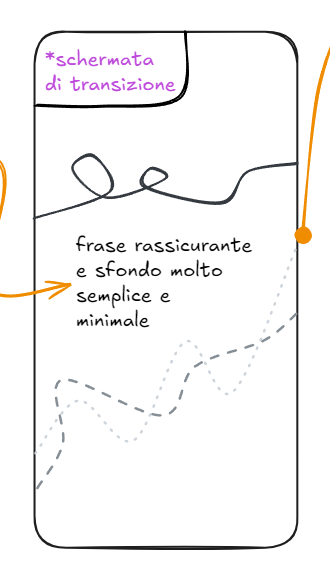
\includegraphics[height=8cm]{imgs/sketches/transizione-s.png}
    \caption{Sketch della schermata di transizione}
    \label{fig:sketch-transizione}
\end{figure}

La schermata è stata quindi ridotta all'essenziale, con una frase rassicurante collocata al centro e uno sfondo appena accennato da linee morbide, privo di pulsanti, di intestazioni e di qualunque elemento di navigazione.
L'assenza totale di comandi è una scelta deliberata, perché in questo passaggio non viene chiesta all'utente alcuna decisione.
Le linee guida di design mettono in guardia dalle schermate di apertura statiche, che interrompono il flusso e sono tra le principali cause di abbandono, e il rischio è stato affrontato limitando la durata a pochi secondi e permettendo di superare la schermata con un tocco.
Il requisito di navigazione reversibile e vie di fuga sicure (\textbf{REQ-03}) esclude infatti esplicitamente le schermate di passaggio dall'obbligo di esporre un comando di uscita, a condizione che si esauriscano da sole e che non trattengano chi vuole procedere.

Al termine della transizione si apre la sequenza vera e propria, composta da tre attività di supporto e da un questionario conclusivo.
Nell'esplorazione le tre schermate sono state disegnate con una struttura comune, in modo che l'utente non debba reimparare l'interfaccia a ogni passaggio.
Nella parte alta un indicatore di avanzamento a tre tappe dichiara il punto del percorso in cui ci si trova, secondo l'annotazione che accompagna gli sketch, mentre accanto ad esso un comando di uscita esplicito permette di interrompere la sessione in qualunque momento (\textbf{REQ-03}).
In basso a sinistra un pulsante informativo mette a disposizione la spiegazione dell'esercizio soltanto a chi la richiede, applicando il principio della formazione fornita nel momento in cui serve anziché anticipata in un tutorial iniziale.
Il fondo della schermata è infine occupato dal comando che conduce al passo successivo, nella posizione più comoda da raggiungere con il pollice.

Questa impostazione non presenta alternative concorrenti, poiché discende dal requisito di fornire strumenti attivi e interattivi per la gestione della crisi (\textbf{REQ-02}) e da quello di garantire una via di uscita costante.
È stata pertanto trasferita integralmente al wireframing, dove è stata verificata schermata per schermata.
Le tre attività e il questionario finale vengono analizzati singolarmente nei paragrafi che seguono.

\subsection{Attività 1: respirazione guidata}
\label{subsec:sketch-respirazione}

La prima attività del percorso è un esercizio di respirazione guidata con tecnica 4-4-4-4, scelto come punto di partenza perché agisce sulla componente fisiologica dell'attacco di panico prima ancora che su quella cognitiva.
Chi sta iperventilando non è nella condizione di ragionare sui propri pensieri, mentre è ancora in grado di seguire un ritmo imposto dall'esterno, e questo rende la respirazione lo strumento più adatto ad aprire la sequenza di soccorso (\textbf{REQ-02}).

\begin{figure}[htbp]
    \centering
    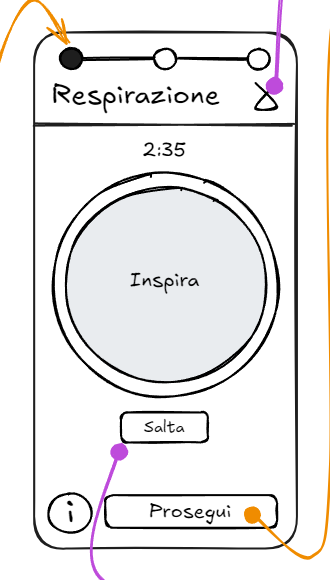
\includegraphics[height=8cm]{imgs/sketches/task-1-s.png}
    \caption{Sketch della respirazione guidata}
    \label{fig:sketch-task1}
\end{figure}

L'elemento centrale della schermata è una circonferenza di grandi dimensioni che si espande e si contrae seguendo le fasi dell'esercizio, accompagnata da una sola parola che dichiara cosa fare in quel momento.
La scelta di affidare la guida a una forma in movimento anziché a un testo descrittivo risponde direttamente al requisito di basso carico cognitivo (\textbf{REQ-01}), poiché un ritmo visivo si imita senza doverlo leggere né interpretare.
Al di sopra della circonferenza un contatore indica il tempo residuo della sessione.
La sua presenza è stata valutata con attenzione, perché le linee guida osservano che un indicatore di avanzamento sposta l'attenzione sull'attesa, ma in questo contesto l'effetto è opposto e desiderabile: sapere che l'esercizio ha una durata definita e visibile rassicura chi teme di essere trattenuto in una procedura senza fine (\textbf{REQ-03}).

La decisione di progetto più significativa riguarda il comando di salto annotato a margine dello sketch, pensato per superare le fasi di trattenimento del respiro.
Un ritmo rigido uguale per tutti si è rivelato inadeguato al contesto, dato che trattenere l'aria durante una crisi respiratoria può risultare faticoso e in alcuni casi accentuare l'affanno anziché ridurlo.
Il comando consente quindi di proseguire nel ciclo saltando la sola pausa, senza abbandonare l'esercizio e senza costringere l'utente a subire una tempistica che il proprio corpo in quel momento non regge.

Il fondo della schermata ospita il comando che conduce all'attività successiva, disponibile in qualunque istante e non vincolato al completamento del contatore.
Nessuno è quindi obbligato a portare a termine l'esercizio per accedere al resto del percorso, coerentemente con il principio di reversibilità che governa l'intero flusso (\textbf{REQ-03}).
L'impostazione è stata trasferita al wireframing senza alternative concorrenti, poiché la metafora della circonferenza pulsante costituisce una convenzione consolidata nelle applicazioni di respirazione guidata e non è parso utile allontanarsene.

\subsection{Attività 2: distrazione cognitiva}
\label{subsec:sketch-distrazione}

La seconda attività sposta l'intervento dal corpo alla mente.
Una volta rallentato il respiro, il problema che resta è il pensiero circolare che alimenta l'attacco, e la strategia adottata consiste nell'occupare l'attenzione con un compito manuale abbastanza semplice da non richiedere alcuno sforzo di comprensione.
Lo sketch la definisce a margine un gioco di distrazione cognitiva, formula che ne descrive con precisione l'intento: interrompere il circolo dei pensieri catastrofici sottraendo loro le risorse attentive necessarie a sostenersi (\textbf{REQ-02}).

\begin{figure}[htbp]
    \centering
    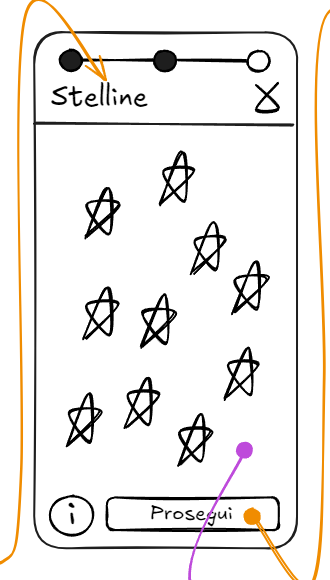
\includegraphics[height=8cm]{imgs/sketches/task-2-s.png}
    \caption{Sketch dell'attività delle stelle}
    \label{fig:sketch-task2}
\end{figure}

L'esercizio consiste nel comporre un cielo notturno accendendo una a una le stelle disseminate sulla schermata.
La distinzione fra le stelle già accese e quelle ancora spente costituisce l'unico riscontro fornito all'utente, e l'attività si conclude quando il cielo è completo oppure quando la persona decide di passare oltre.
Il compito richiede una ricerca visiva e un gesto di puntamento sufficientemente preciso da assorbire l'attenzione, ma ogni tocco produce un risultato immediato e visibile, senza che sia mai necessario ricordare una regola o pianificare una mossa.

Nella definizione di questa attività la scelta più delicata è stata quella di rinunciare a qualsiasi meccanica competitiva.
Un gioco dotato di punteggio, di limite di tempo o di condizione di sconfitta avrebbe introdotto una possibilità di fallimento, e chiedere prestazioni a una persona nel mezzo di un attacco di panico avrebbe aggiunto ansia invece di sottrarne.
Il compito è stato quindi costruito in modo che non esista un modo sbagliato di svolgerlo, e la sua unica ricompensa è di natura estetica, ovvero il cielo che si completa progressivamente sotto le dita dell'utente.

La disposizione irregolare delle stelle risponde infine a una necessità pratica oltre che visiva.
Le dita sono strumenti di puntamento imprecisi e lo diventano ulteriormente quando il tremore accompagna la crisi, per cui gli elementi interattivi sono stati dimensionati con generosità e distanziati fra loro, in modo che un tocco approssimativo raggiunga comunque il bersaglio previsto.
L'attività è stata trasferita al wireframing senza alternative concorrenti, poiché nessuna delle varianti considerate durante l'esplorazione univa altrettanto bene la semplicità del gesto all'assenza di qualsiasi pressione sull'utente.

\subsection{Attività 3: grounding 5-4-3-2-1}
\label{subsec:sketch-grounding}

La terza attività chiude la sequenza riportando l'attenzione sull'ambiente circostante.
La tecnica 5-4-3-2-1 chiede di individuare e nominare cinque cose che si vedono, quattro che si toccano, tre che si sentono, due che si annusano e una che si gusta, costruendo una scala che sposta progressivamente il fuoco dall'interno del corpo al mondo esterno.
Rispetto alle due attività precedenti il ruolo dell'interfaccia cambia in modo sostanziale, poiché qui l'applicazione non fornisce nulla da guardare o da toccare sullo schermo ma si limita a scandire un compito che si svolge interamente nella stanza in cui l'utente si trova (\textbf{REQ-02}).

\begin{figure}[htbp]
    \centering
    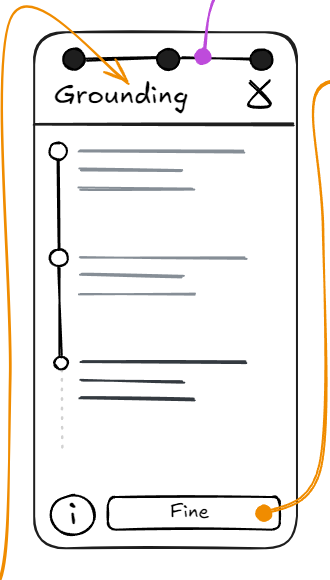
\includegraphics[height=8cm]{imgs/sketches/task-3-s.png}
    \caption{Sketch del grounding 5-4-3-2-1}
    \label{fig:sketch-task3}
\end{figure}

La decisione di progetto centrale riguarda il modo in cui i cinque passaggi vengono presentati.
Mostrarli tutti insieme avrebbe trasformato la schermata in un elenco di istruzioni da leggere e da tenere a mente, esattamente il tipo di carico che il requisito di interfaccia minimale impone di evitare (\textbf{REQ-01}).
Gli sketch adottano quindi una rivelazione progressiva lungo una linea verticale, nella quale compare un passaggio alla volta e l'utente avanza soltanto quando si sente pronto.
In questo modo la persona ha davanti a sé una sola richiesta per volta, formulata con poche parole e priva di qualsiasi ramificazione.

I passaggi già completati rimangono visibili al di sopra di quello corrente, resi in una tonalità attenuata che ne dichiara la conclusione senza cancellarli.
La scelta consente di rileggere ciò che si è appena fatto e restituisce la misura concreta del percorso compiuto, aspetto tutt'altro che secondario per chi fatica a percepire il passare del tempo durante una crisi.
I passaggi non ancora raggiunti sono invece accennati da segnaposto grigi, secondo il principio delle schermate scheletro descritto nelle linee guida, che sposta l'attenzione sul progredire del contenuto ed evita che l'interfaccia sembri terminare dove finisce il testo visibile.

A differenza della respirazione guidata, questa attività non prevede alcun contatore e nessuna durata prestabilita.
Il tempo necessario a individuare cinque oggetti dipende dall'ambiente in cui ci si trova e dalla lucidità del momento, e imporre un ritmo uniforme avrebbe trasformato un esercizio di osservazione in una prova a tempo.
L'avanzamento è pertanto affidato interamente al comando premuto dall'utente, mentre la conclusione della scala conduce al questionario finale.
L'impostazione è stata trasferita al wireframing senza alternative concorrenti.

\subsection{Attività conclusiva: questionario di feedback}
\label{subsec:sketch-questionario}

La sequenza si chiude con un questionario che raccoglie il resoconto di quanto appena accaduto.
La collocazione al termine del percorso non è casuale, poiché il ricordo di un attacco di panico si sbiadisce rapidamente e la sua intensità viene ridimensionata a distanza di ore.
L'analisi dei competitor aveva evidenziato proprio in questo punto una lacuna significativa, dal momento che il tracciamento vi risulta possibile soltanto nei momenti di calma, con la conseguenza di perdere il legame fra lo stato emotivo registrato e l'episodio che lo ha provocato.
Chiedere le stesse informazioni subito dopo la crisi permette invece di raccoglierle mentre sono ancora nitide (\textbf{REQ-06}).

\begin{figure}[htbp]
    \centering
    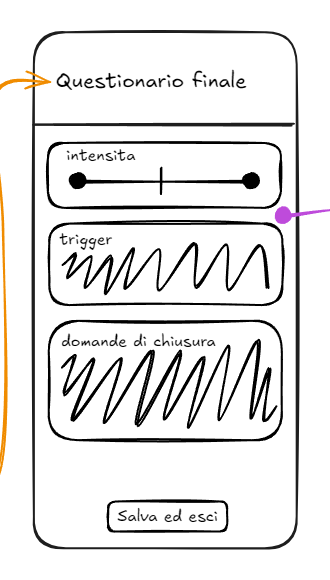
\includegraphics[height=8cm]{imgs/sketches/questionario-s.png}
    \caption{Sketch del questionario di chiusura}
    \label{fig:sketch-questionario}
\end{figure}

Il vincolo che ha guidato la progettazione di questa schermata è la condizione di chi la incontra, ovvero una persona appena uscita da un attacco, stanca e poco disposta a compilare moduli.
Ogni domanda è stata quindi ridotta a un gesto anziché a una digitazione.
Lo sketch dispone verticalmente tre blocchi, nei quali l'intensità dell'attacco si dichiara facendo scorrere un cursore lungo una scala graduata, mentre il fattore scatenante e le domande di chiusura occupano due riquadri distinti la cui forma definitiva è stata rimandata alla fase successiva.
L'annotazione a margine si limita infatti a registrare la necessità di un modo per descrivere l'evento che ha innescato la crisi, lasciando aperta la scelta fra una descrizione scritta e una selezione fra opzioni già disponibili.

La schermata si conclude con il comando che salva le risposte e riporta alla schermata principale, unico punto dell'intero flusso in cui il salvataggio viene dichiarato in modo esplicito.
Questa formulazione rende evidente che i dati raccolti vengono conservati nel diario, dove alimentano lo storico consultabile (\textbf{REQ-07}) e la sintesi settimanale dell'andamento (\textbf{REQ-09}).
Anche in questo caso non sono state disegnate alternative concorrenti, e l'impostazione è stata trasferita al wireframing così come esplorata.

\section{Schermata Diario: tracking delle crisi e riflessione personale}
\label{sec:sketch-diario}

Il diario raccoglie tutto ciò che l'applicazione registra nel tempo e costituisce la sede in cui il requisito di storico consultabile (\textbf{REQ-07}) prende forma concreta.
In fase esplorativa la difficoltà principale non è stata decidere quali informazioni conservare, già stabilite dai requisiti, ma trovare un criterio che le tenesse insieme senza disperderle in sezioni separate.
La soluzione adottata assume la giornata come unità di aggregazione, secondo l'annotazione a margine dello sketch che descrive l'obiettivo di racchiudere a prima vista, e giorno per giorno, tutte le informazioni necessarie all'utente.

\begin{figure}[htbp]
    \centering
    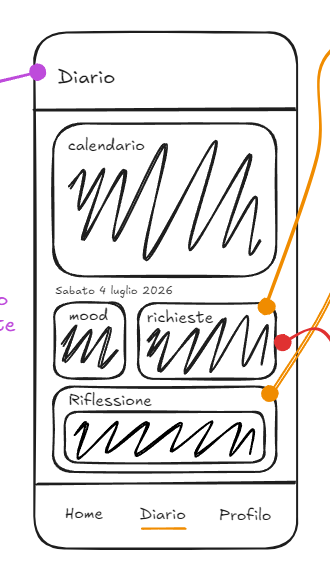
\includegraphics[height=8cm]{imgs/sketches/diario-s.png}
    \caption{Sketch del diario, con il calendario e il riepilogo della giornata}
    \label{fig:sketch-diario}
\end{figure}

La schermata si apre quindi con un calendario mensile che occupa la porzione superiore e funziona da selettore, permettendo di raggiungere qualunque giornata già trascorsa senza attraversare elenchi intermedi.
Alla selezione di una data la parte sottostante si aggiorna mostrando il riepilogo corrispondente, articolato in tre card affiancate o sovrapposte: l'umore registrato quel giorno (\textbf{REQ-06}), l'elenco delle richieste di aiuto avvenute (\textbf{REQ-07}) e la riflessione scritta dall'utente (\textbf{REQ-10}).

L'impostazione evita che l'utente debba ricostruire da solo la relazione fra dati che appartengono allo stesso momento.
Un attacco di panico, l'umore dichiarato quella mattina e le parole scritte in serata sono episodi collegati, e separarli in schermate distinte avrebbe costretto a una navigazione ripetuta per ottenere un quadro che invece deve presentarsi in un colpo d'occhio.
Il ricorso alle card mantiene inoltre riconoscibile il confine fra le tre informazioni, senza che il riepilogo si trasformi in un elenco indistinto.

Poiché ciascuna delle tre card dispone di uno spazio necessariamente limitato, l'esplorazione ha previsto che le richieste di aiuto e la riflessione potessero essere aperte in una vista dedicata, richiamabile con un tocco sulla card corrispondente.
Il calendario e la struttura del riepilogo sono stati trasferiti al wireframing senza modifiche sostanziali, mentre per la vista di dettaglio delle richieste sono state disegnate due alternative, discusse nel paragrafo seguente.

\subsection{Richieste di supporto: vista di dettaglio}
\label{subsec:sketch-richieste}

La card delle richieste di aiuto inserita nel riepilogo giornaliero dispone di uno spazio ridotto, sufficiente a segnalare che quel giorno si sono verificati degli episodi ma non a descriverli.
Per consultarli è stata quindi prevista una vista dedicata, richiamabile con un tocco sulla card, nella quale ogni richiesta espone l'orario in cui è avvenuta, l'intensità dichiarata e il fattore scatenante indicato al termine della sessione (\textbf{REQ-07}).
Per questa vista sono state disegnate due alternative che differiscono nel modo di rappresentare il singolo episodio.

\begin{figure}[htbp]
    \centering
    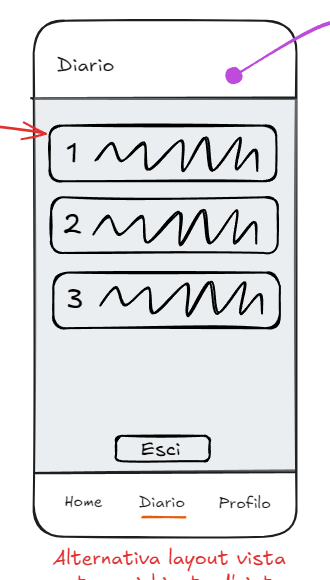
\includegraphics[height=8cm]{imgs/sketches/popup-richieste-aiuto-s.png}\hspace{1cm}
    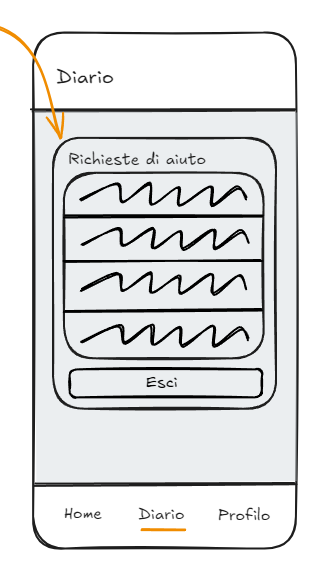
\includegraphics[height=8cm]{imgs/sketches/popup-richieste-aiuto-alt-s.png}
    \caption{Le due alternative per la vista di dettaglio delle richieste di aiuto}
    \label{fig:sketch-richieste}
\end{figure}

La prima variante assegna a ogni richiesta un blocco autonomo, numerato progressivamente e disteso su tutta la larghezza dello schermo.
La generosità dello spazio permette di leggere senza sforzo i dati di ciascun episodio e di distinguerli a colpo d'occhio, ma la stessa impostazione mostra il proprio limite nelle giornate difficili.
Quando gli attacchi sono stati numerosi l'elenco si allunga oltre l'altezza della schermata e i blocchi, separati l'uno dall'altro, finiscono per apparire come oggetti indipendenti anziché come le voci di un unico registro, indebolendo la percezione di continuità che il diario dovrebbe restituire.

La seconda variante raccoglie invece tutte le richieste all'interno di un solo contenitore, disponendole come righe compatte e sovrapposte.
La densità informativa cresce sensibilmente, poiché un numero maggiore di episodi resta visibile contemporaneamente, e la forma richiama quella già impiegata nella card del riepilogo, rafforzando la coerenza interna dell'applicazione.
Il vantaggio comporta però una contropartita, dal momento che l'altezza ridotta di ciascuna riga limita la quantità di informazioni esponibili e avvicina la vista all'aspetto di una tabella, con il rischio che i singoli episodi si confondano in un elenco indistinto.

L'annotazione a margine dello sketch riconosce alla prima proposta una minore adeguatezza, ma dichiara insieme che in quella fase era ancora presto per decidere, poiché il confronto teorico non bastava a stabilire quanto la maggiore leggibilità del blocco autonomo pesasse rispetto alla compattezza dell'elenco.
Entrambe le alternative sono state pertanto conservate e tradotte in wireframe, per essere confrontate empiricamente nella successiva valutazione con gli utenti.

\subsection{Spazio sicuro: la riflessione personale}
\label{subsec:sketch-riflessione}

L'ultima delle tre card del riepilogo giornaliero ospita lo spazio di scrittura libera, l'unico punto dell'applicazione in cui l'utente si esprime con parole proprie anziché scegliere fra opzioni predefinite (\textbf{REQ-10}).
Come per le richieste di aiuto, l'anteprima contenuta nel riepilogo serve soltanto a segnalare la presenza di un testo, mentre la scrittura e la rilettura avvengono in una vista dedicata che si apre con un tocco sulla card.

\begin{figure}[htbp]
    \centering
    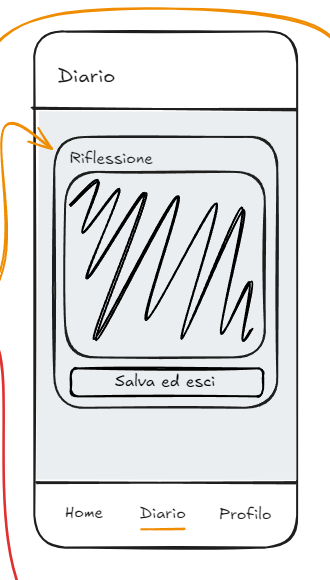
\includegraphics[height=8cm]{imgs/sketches/popup-riflessione-s.png}
    \caption{Sketch della riflessione personale}
    \label{fig:sketch-riflessione}
\end{figure}

La schermata destina quasi l'intera altezza disponibile all'area di testo, alla quale restano attorno soltanto il titolo, il comando di salvataggio e la barra di navigazione comune al resto dell'applicazione.
La scelta risponde alla natura dell'attività, poiché mettere in parole un'esperienza di sofferenza richiede una concentrazione che qualsiasi elemento accessorio finirebbe per interrompere.
Ogni componente non indispensabile è stato quindi rimosso, in coerenza con il requisito di interfaccia minimale (\textbf{REQ-01}) e con l'indicazione delle linee guida di ridurre al minimo la cornice grafica quando l'utente deve concentrarsi su un compito principale.

Altrettanto deliberata è l'assenza di qualsiasi struttura imposta al testo.
Non sono previsti strumenti di formattazione, domande guida, modelli da completare o limiti di lunghezza, perché suggerire un argomento significherebbe orientare ciò che la persona scrive e costringere il suo vissuto entro categorie stabilite da altri.
Lo spazio si presenta quindi vuoto e privo di indicazioni, disponibile tanto per poche righe quanto per un racconto disteso, e resta modificabile anche in un momento successivo, poiché la lucidità necessaria a rileggersi arriva spesso a distanza di ore dall'episodio.

La schermata si chiude con un comando esplicito che salva il testo e riporta al diario.
La formulazione, che dichiara insieme il salvataggio e l'uscita, evita l'ambiguità di un semplice comando di chiusura, dal quale l'utente non potrebbe dedurre se quanto scritto verrà conservato oppure perduto.
Il requisito di navigazione reversibile chiede infatti che le conseguenze di un abbandono siano dichiarate prima che questo avvenga (\textbf{REQ-03}).
L'impostazione non presenta alternative concorrenti ed è stata trasferita al wireframing così come esplorata.

\section{Schermata Profilo: dati utente e preferenze di notifica}
\label{sec:sketch-profilo}

Il profilo occupa la terza scheda della barra di navigazione ed è l'unica area dell'applicazione che non interviene nella gestione della crisi.
Vi confluiscono i dati anagrafici dell'account, le preferenze di funzionamento e i comandi che agiscono sull'archivio personale, ovvero tutto ciò che una persona consulta di rado e sempre in condizioni di calma.
Questa differenza di contesto ha permesso di adottare una densità informativa superiore rispetto alle altre schermate, senza contraddire il requisito di interfaccia minimale, che riguarda i momenti di vulnerabilità e non l'intera applicazione (\textbf{REQ-01}).

\begin{figure}[htbp]
    \centering
    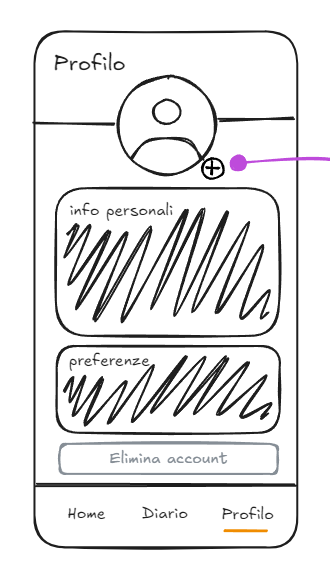
\includegraphics[height=8cm]{imgs/sketches/profilo-s.png}
    \caption{Sketch del profilo}
    \label{fig:sketch-profilo}
\end{figure}

La schermata si apre con l'immagine dell'utente, alla quale è affiancato un comando dedicato alla sua sostituzione, come indicato dall'annotazione a margine dello sketch.
Al di sotto si susseguono due blocchi distinti, il primo destinato ai dati personali inseriti in fase di registrazione e il secondo alle preferenze, dove trova posto l'attivazione del promemoria quotidiano (\textbf{REQ-12}).
La separazione in blocchi consente di distinguere a colpo d'occhio ciò che descrive l'utente da ciò che regola il comportamento dell'applicazione.

La decisione di progetto più delicata riguarda l'eliminazione dell'account, comando che il requisito di riservatezza impone di rendere disponibile, poiché a chi ha creato un profilo deve restare la possibilità di cancellare l'intero archivio in qualsiasi momento (\textbf{REQ-05}).
Lo stesso comando è però l'unico dell'applicazione a produrre una perdita irreversibile di dati, e le linee guida raccomandano di collocare le azioni distruttive al di fuori della zona raggiungibile senza intenzione.
Nello sketch è stato quindi isolato in fondo alla schermata, oltre i blocchi che raccolgono le funzioni ordinarie, e disegnato con un contorno privo di riempimento che ne abbassa il peso visivo rispetto agli altri comandi.

L'accostamento fra le due esigenze si risolve così senza sacrificarne nessuna, dal momento che il comando resta presente e individuabile da chi lo cerca, ma non compete per l'attenzione di chi sta semplicemente consultando i propri dati.
Anche in questo caso non sono state esplorate alternative concorrenti, poiché l'organizzazione per blocchi tematici costituisce una convenzione consolidata per le schermate di impostazioni, e l'impostazione è stata trasferita al wireframing così come disegnata.

\section{Mappa delle transizioni e flusso di aiuto}
\label{sec:sketch-mappa}

Gli sketch esaminati fino a questo punto descrivono le singole schermate, ma non dicono nulla su come si raggiungano l'una dall'altra.
Per questa ragione l'esplorazione non è stata condotta su fogli separati, bensì disponendo tutte le interfacce su un'unica superficie e tracciando direttamente su di essa i collegamenti fra loro.
La rappresentazione che ne risulta corrisponde a quanto le linee guida descrivono come flusso delle attività, ovvero la sequenza di schermate attraverso cui l'utente passa per portare a termine un compito, e costituisce il complemento naturale dei prototipi appena presentati.

Sul foglio convivono tre tipi di segno, ciascuno con una funzione distinta.
Le frecce arancioni rappresentano le transizioni effettive fra le schermate e permettono di seguire un percorso dall'inizio alla fine senza ricostruirlo a memoria.
I segni rossi collegano invece una schermata alla propria variante alternativa e ne dichiarano l'esito, come nel caso del layout della schermata principale contrassegnato come scartato.
Le annotazioni viola, infine, non descrivono movimenti ma motivazioni, e registrano accanto all'elemento interessato la ragione di una scelta oppure il difetto che ne ha determinato l'abbandono.

La lettura d'insieme rende immediatamente visibile la struttura di navigazione dell'applicazione.
Dalle tre aree raggiungibili con la barra inferiore si diramano percorsi di natura differente, poiché il diario apre viste di dettaglio dalle quali si torna indietro, mentre il pulsante di aiuto avvia una sequenza lineare che attraversa la transizione, le tre attività e il questionario conclusivo.
Proprio in questa sequenza le schermate sono state disegnate senza la barra di navigazione, scelta che sul foglio appare con particolare evidenza e che dichiara l'intenzione di isolare il percorso di soccorso dal resto dell'applicazione.

Le linee guida raccomandano di non costruire un unico flusso che pretenda di contenere l'intero sistema, ma di concentrarsi sugli scenari principali.
Nel caso di Vivo l'architettura è risultata sufficientemente contenuta da poter essere rappresentata per intero senza compromettere la leggibilità, e mantenere ogni cosa sotto lo stesso sguardo ha permesso di valutare simultaneamente le transizioni, le alternative in competizione e le motivazioni annotate.
La mappa ha così confermato la struttura di navigazione adottata e ha costituito il punto di partenza della successiva traduzione in wireframe.

\begin{figure}[htbp]
    \centering
    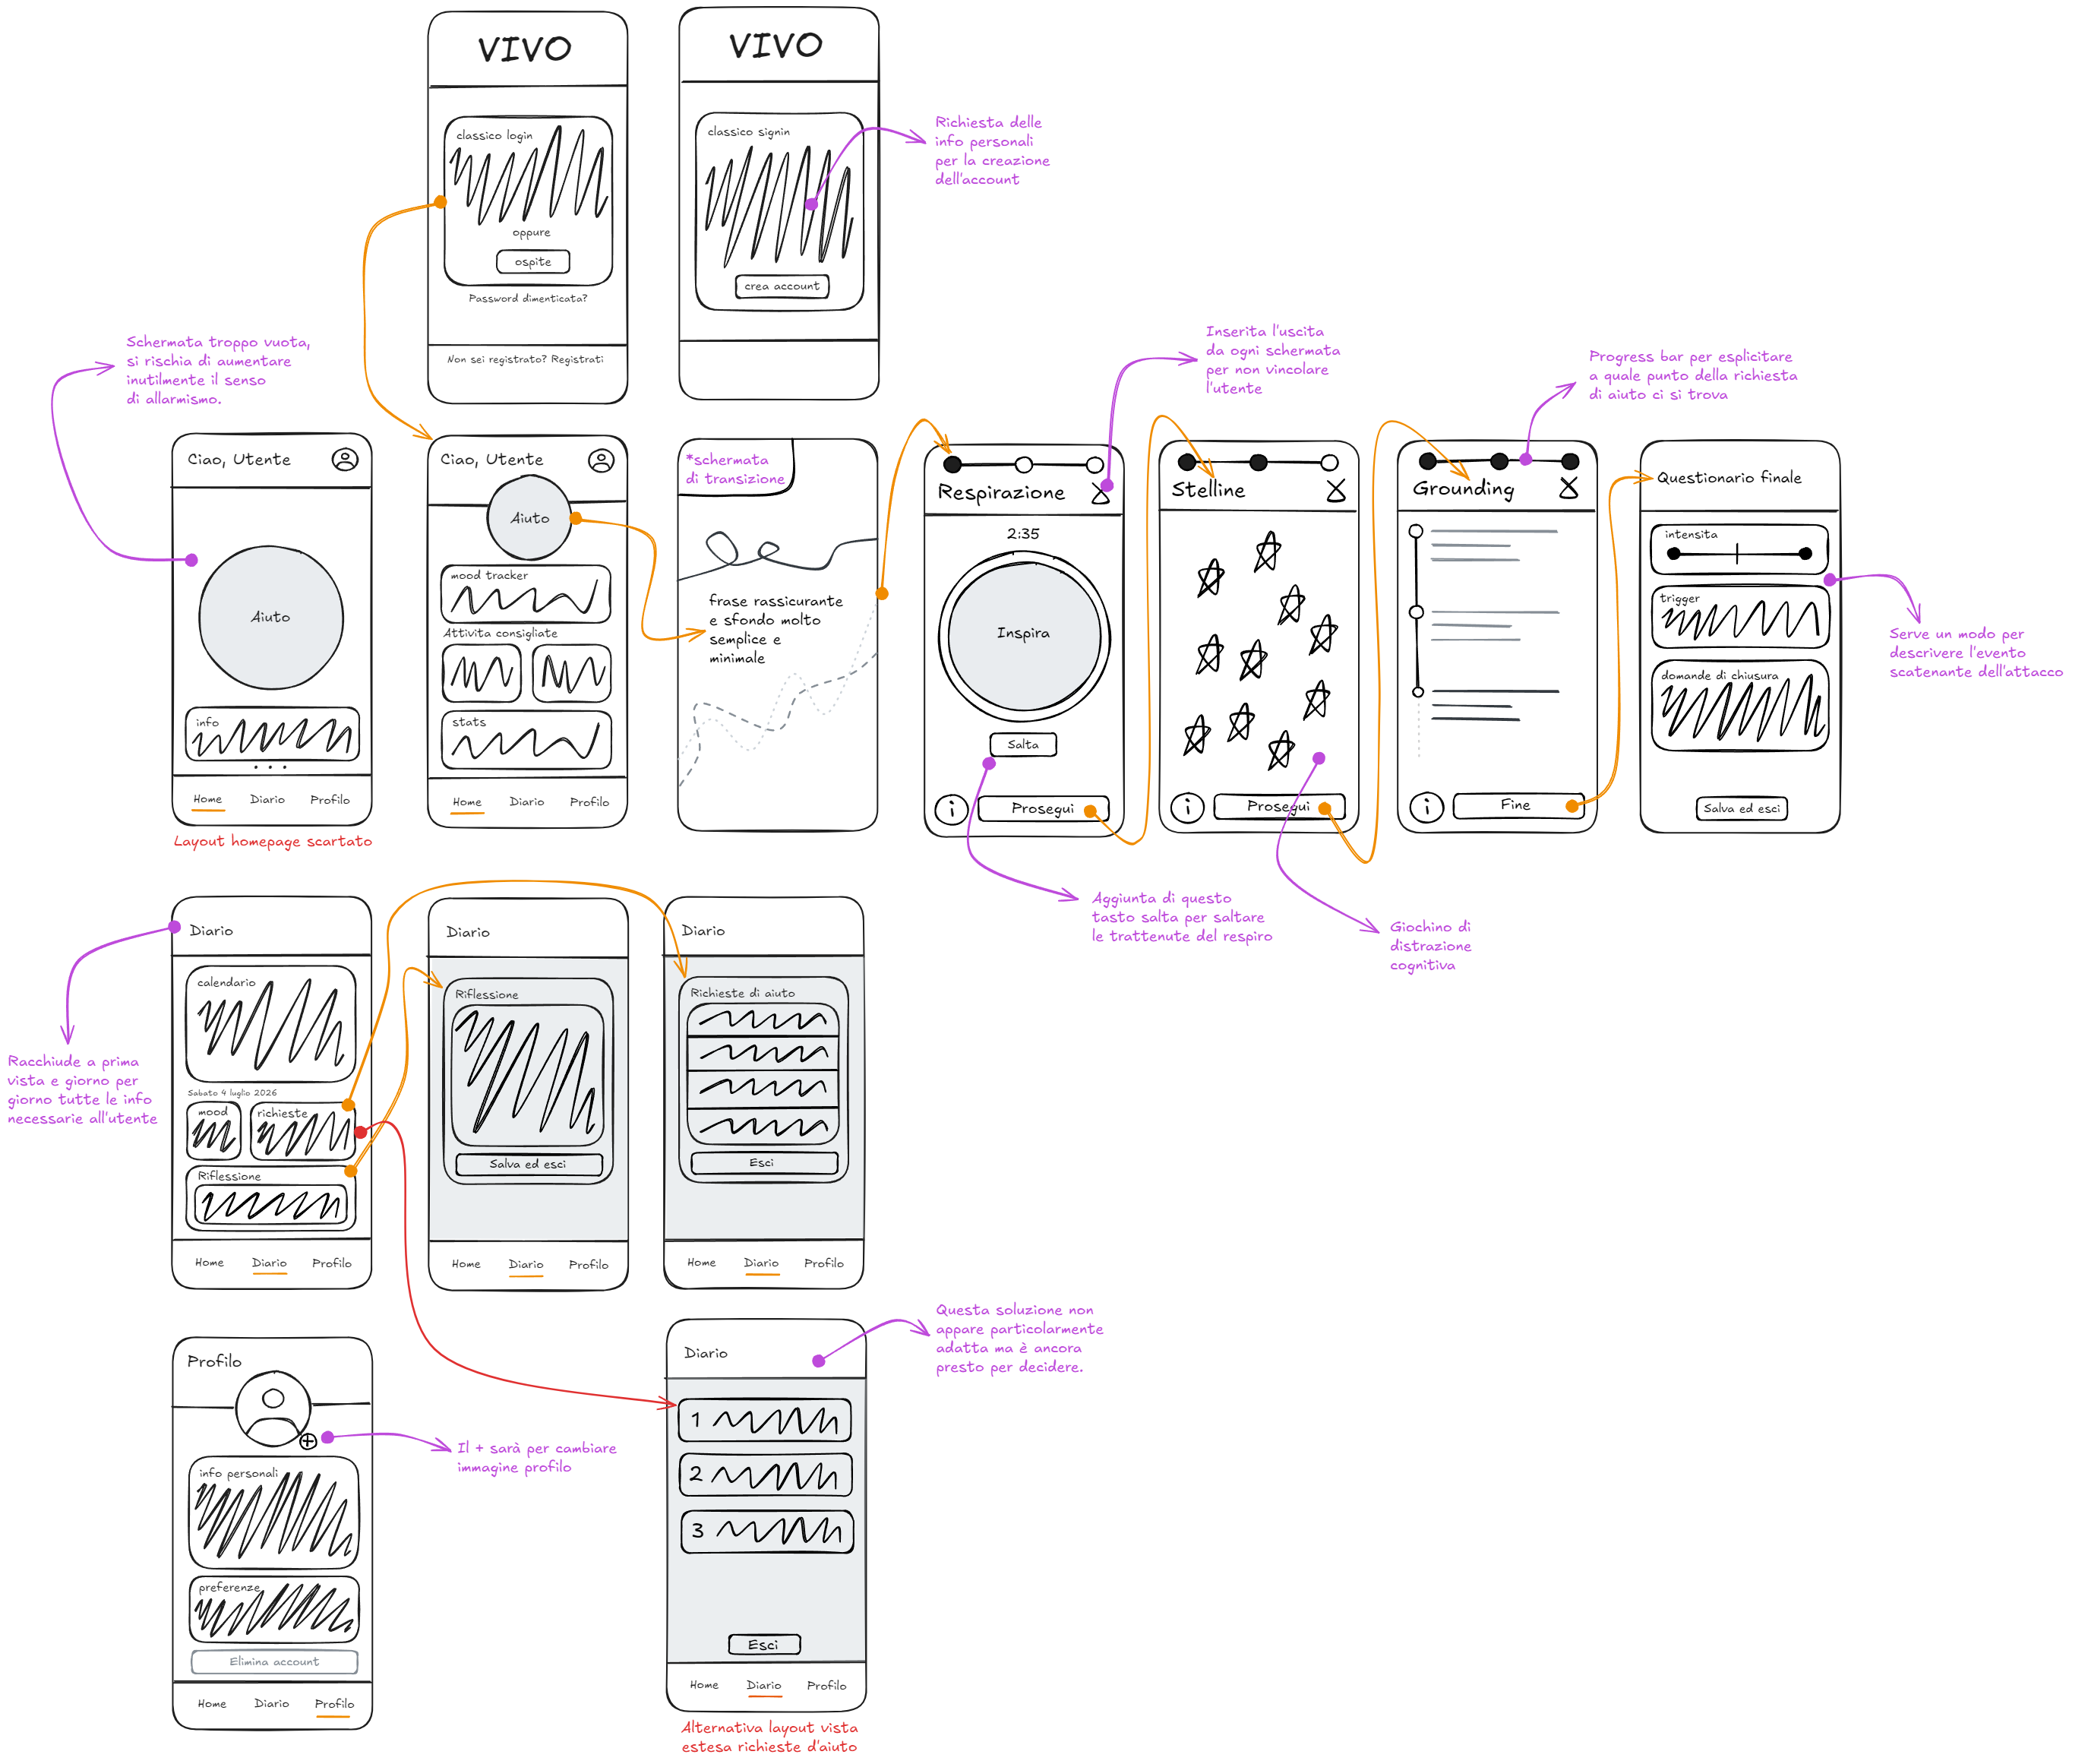
\includegraphics[width=\textwidth]{imgs/sketches/sketch-tot.png}
    \caption{Il foglio completo degli sketch: in arancione le transizioni, in rosso le alternative in competizione, in viola le motivazioni annotate}
    \label{fig:sketch-totale}
\end{figure}
